% Created 2021-10-24 Sun 14:32
% Intended LaTeX compiler: pdflatex
\documentclass[11pt]{article}
\usepackage[utf8]{inputenc}
\usepackage[T1]{fontenc}
\usepackage{graphicx}
\usepackage{grffile}
\usepackage{longtable}
\usepackage{wrapfig}
\usepackage{rotating}
\usepackage[normalem]{ulem}
\usepackage{amsmath}
\usepackage{textcomp}
\usepackage{amssymb}
\usepackage{capt-of}
\usepackage{hyperref}
\author{Amalkrishnaur}
\date{\today}
\title{}
\hypersetup{
 pdfauthor={Amalkrishnaur},
 pdftitle={},
 pdfkeywords={},
 pdfsubject={},
 pdfcreator={Emacs 26.3 (Org mode 9.1.9)}, 
 pdflang={English}}
\begin{document}

\tableofcontents

\section{What is space?}
\label{sec:org0f0bbde}
\begin{itemize}
\item When we think of space we think about space where we live but in mathematics it more then that 
In mathamatics any generic abstract collection of elements are called space
\end{itemize}
\section{Function Space}
\label{sec:org429cc98}
\begin{itemize}
\item Space of all possible function F(x)
\item Idea is come from linear algebra
\item It is like vector space with infinit dimenstions
\end{itemize}
\subsection{Hilbert space}
\label{sec:org4c60f8c}
Space all possible wave functions
\section{Vectors}
\label{sec:org480e258}
\begin{figure}[htbp]
\centering
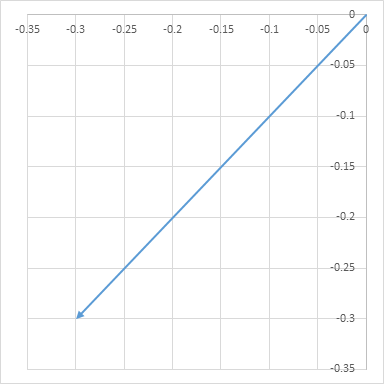
\includegraphics[width=.9\linewidth]{./2d-vector-grapher-8.png}
\caption{\label{fig:org66145ef}
This is Vector}
\end{figure}
\begin{itemize}
\item It has both dirction and magnitude
\end{itemize}
\subsection{Vectors}
\label{sec:org1ac6d76}
\begin{center}
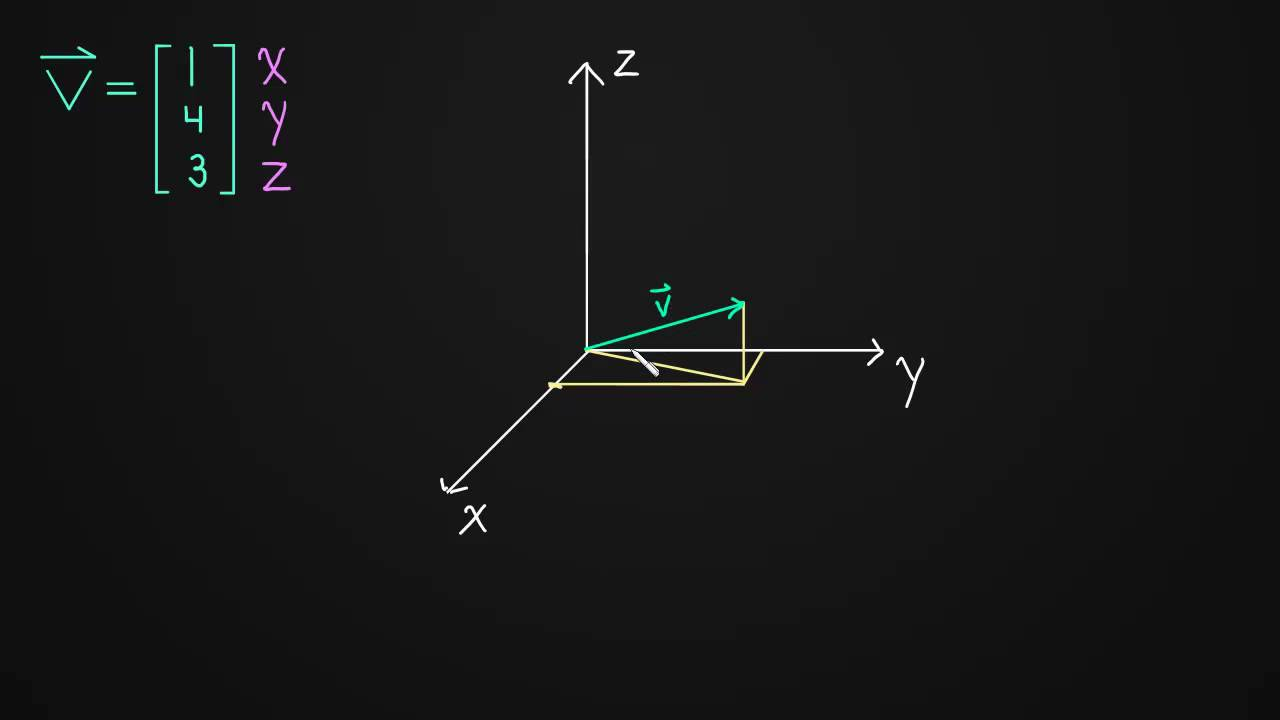
\includegraphics[width=.9\linewidth]{./vect.jpg}
\end{center}
\subsection{Component reprasentation}
\label{sec:orgbe9e827}
\begin{itemize}
\item \(\vec a\) = x\(\hat i\) + y\(\hat j\) + z \(\hat k\)
\item Also i can write this way
\item \(\vec a\) = \(\frac{\vec a . \hat i}{||\hat i||^2}\) + \(\frac{\vec a . \hat j}{||\hat j||^2}\) + \(\frac{\vec a . \hat k}{||\hat k||^2}\)
\end{itemize}
\section{cordinate transformation}
\label{sec:orgcd258ff}
\begin{center}
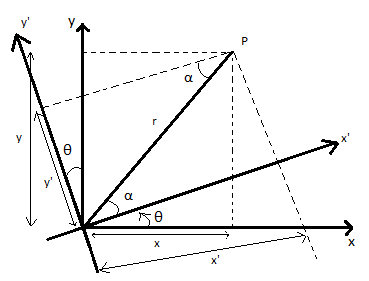
\includegraphics[width=.9\linewidth]{./ct.png}
\end{center}
\subsection{cordinate transformation}
\label{sec:orgdba758f}
\begin{itemize}
\item I can write p interms of x and y
\item \(\vec p\) = \(\frac{\vec p . x}{||x||^2}\) + \(\frac{\vec p . y }{||y||^2}\)
\item I can alse write in terms of x' and y'
\item \(\vec p\) = \(\frac{\vec p . x'}{||x'||^2}\) + \(\frac{\vec p . y' }{||y'||^2}\)
\item here dot product give projection on to each axis and tell how much that vector in point in x dirction
\item Also when dot product is zero the vectors are in orthogonal to each other
\end{itemize}
\section{Inner product of functions}
\label{sec:org471aeb0}
\begin{itemize}
\item It is just like dot product between two vectors
\item A function can be thought as vector of infinit dimenstion
\item For defining innerproduct just descritize our functions f and g in some intervel a and b
\item We have \(\begin{bmatrix}f_1 & f_2 & \ldots & f_n \end{bmatrix}\) and 
\(\begin{bmatrix}g_1 & g_2 & \ldots & g_n \end{bmatrix}\) Now we can find innerproduct of this it just two vectors
\end{itemize}
\subsection{Inner product continue}
\label{sec:org2f9a315}
\begin{itemize}
\item Now the innerproduct is
\item \[\sum_{k=0}^{n-1} f_kg_k\]
\item This as one problem when n increses this changes by huge amound so we need to normalize this by \(\Delta\) x
\end{itemize}
\subsection{Inner product continue}
\label{sec:orga80abb4}
\begin{itemize}
\item Now after normalization by \(\Delta\) x the equation become
\item \[\sum_{k=0}^{n-1} f_kg_k\Delta x\]
\item This is Riemann approximation of inegral
\end{itemize}
\subsection{Innerproduct}
\label{sec:org171eaea}
\begin{itemize}
\item Now the equation become
\item <f(x),g(x)> = \(\int_a^b\) f(x)g(x) dx
\end{itemize}
\subsection{Inner product matlab}
\label{sec:org4c4737c}
\begin{verbatim}
clear all, close all, clc

f = [0 0 .1 .2  .25  .2 .25 .3 .35 .43 .45 .5 .55  .5 .4 .425 .45 .425 .4 .35 .3 .25 .225 .2 .1 0 0];
g = [0 0 .025 .1  .2  .175 .2 .25 .25 .3 .32 .35 .375  .325 .3 .275 .275 .25 .225 .225 .2 .175 .15 .15 .05 0 0] -0.025;

x = 0.1*(1:length(f));

xf = (.01:.01:x(end));
ff = interp1(x,f,xf,'cubic')

gf = interp1(x,g,xf,'cubic')


plot(xf(20:end-10),ff(20:end-10),'k','LineWidth',1.5)
hold on
plot(x(2:end-1),f(2:end-1),'bo','MarkerFace','b')
plot(xf(20:end-10),gf(20:end-10),'k','LineWidth',1.5)
plot(x(2:end-1),g(2:end-1),'ro','MarkerFace','r')


xlim([.1 2.7])
ylim([-.1 .6])
set(gca,'XTick',[.2:.1:2.6],'XTickLabels',{},'LineWidth',1.2)
set(gca,'YTick',[]);
box off

set(gcf,'Position',[100 100 550 250])

set(gcf,'PaperPositionMode','auto')
print('-depsc2', '-loose', '../figures/InnerProduct');

% %%
% xc = x;
% fc = f;
% n = length(x);
% hold on
% fapx = 0*ff;
% dx = xc(2)-xc(1);
% L = xc(end)-xc(1);
% L = 2.5
% A0 = (1/pi)*sum(fc.*ones(size(xc)))*dx*L;
% fapx = fapx + A0/2;
% for k=1:10
%     Ak = (1/pi)*sum(fc.*cos(2*pi*k*xc/L))*dx*L;
%     Bk = (1/pi)*sum(fc.*sin(2*pi*k*xc/L))*dx*L;
% 
%     fapx = fapx + Ak*cos(2*k*pi*xf/L) + Bk*sin(2*k*pi*xf/L);
% end
%     plot(xf,fapx,'k')

\end{verbatim}
\section{Orthogonal Functions}
\label{sec:org2a83b2d}
\begin{itemize}
\item In vectors to check orthogonality we do dot product if dot product is zero then the vectors is orthogonal to each other
\item \(\vec a.\vec b\) = |a||b|cos(\(\theta\)) = 0
\item mean \(\theta\) = 90\(^{\circ}\)
\item In functions we can do the same thing
\end{itemize}
\subsection{Orthogonal Functions continue}
\label{sec:org5a4197e}
\begin{itemize}
\item In function space if f and g are orthogonal to each other then innerproduct is zero
\item \(\int_a^{b}\) f(x)g(x) dx = 0
\end{itemize}
\subsection{Why Importent}
\label{sec:org3baff67}
\begin{itemize}
\item In vectorspace we represents vectors in terms of orthogonal basis
\item Same can do in Function Space Represent any function interms of orthogonal functions
\item One example of this is Fourier Transform
\item It reprasent f(x) interms of orthogonal sins and cosins
\end{itemize}
\section{Fourier Series}
\label{sec:orgbdce917}
\begin{itemize}
\item It is a cordinate transformation
\item It is made for solving heat equation in 1800s
\item It decompose the signal f into sins and cosins
\item sins and cosins are form a orthogonal basis for function space
\end{itemize}
\subsection{Fourier Series}
\label{sec:org0d8a3cc}
\begin{itemize}
\item Any periodic signals can be reprasent interms of sum of sins and cosins
\item \[f(x) = \frac{A_0}{2} + \sum_{k=1}^{\infty} (A_k Cos(kx) + B_k Sin(kx))\]
\end{itemize}
\subsection{FS continue}
\label{sec:org04218ee}
\begin{itemize}
\item It can be thought as ths
\item f(x) = \(\sum_{k=0}^{\infty}\) (<f(x),cos(kx)> \(\frac{cos(kx)}{||cos(kx)||^2}\) + <f(x),sin(kx)> \(\frac{sin(kx)}{||sin(kx)||^2}\))
\end{itemize}
\subsection{Fs}
\label{sec:org2a7b4b8}
\begin{itemize}
\item A\(_{\text{k}}\) = \(\frac{1}{||cos(kx)||^2}\) <f(x),cos(kx)>
\item B\(_{\text{k}}\) = \(\frac{1}{||sin(kx)||^2}\) <f(x),sin(kx)>
\item ||f(x)||\(^{\text{2}}\) = <f(x),f(x)>
\end{itemize}

\subsection{Complex Fourier Series}
\label{sec:org6c276d2}
\begin{itemize}
\item it uses complex exponential to reprasent signal
\item Coefficient can be found exactly same as that of fourier series
\item project function into each complex exponential basis you get the coefficient c\(_{\text{k}}\)
\end{itemize}
\subsection{Reprasentation}
\label{sec:orgb584734}
\begin{itemize}
\item \[ f(x) =  \sum_{k=-\infty}^{\infty}  C_k e^{j\omega_0 kt}\]
\item C\(_{\text{k}}\) = \(\frac{1}{2\pi}\) <f(x),e\(^{\text{jk}\omega_{\text{0}} \ \text{t}}\)>
\end{itemize}
\subsection{Example}
\label{sec:org2e3cead}
\begin{itemize}
\item Assume we have a signal f(x) = 3sin(x) + 3cos(x) then it will look like this
\end{itemize}
\begin{center}
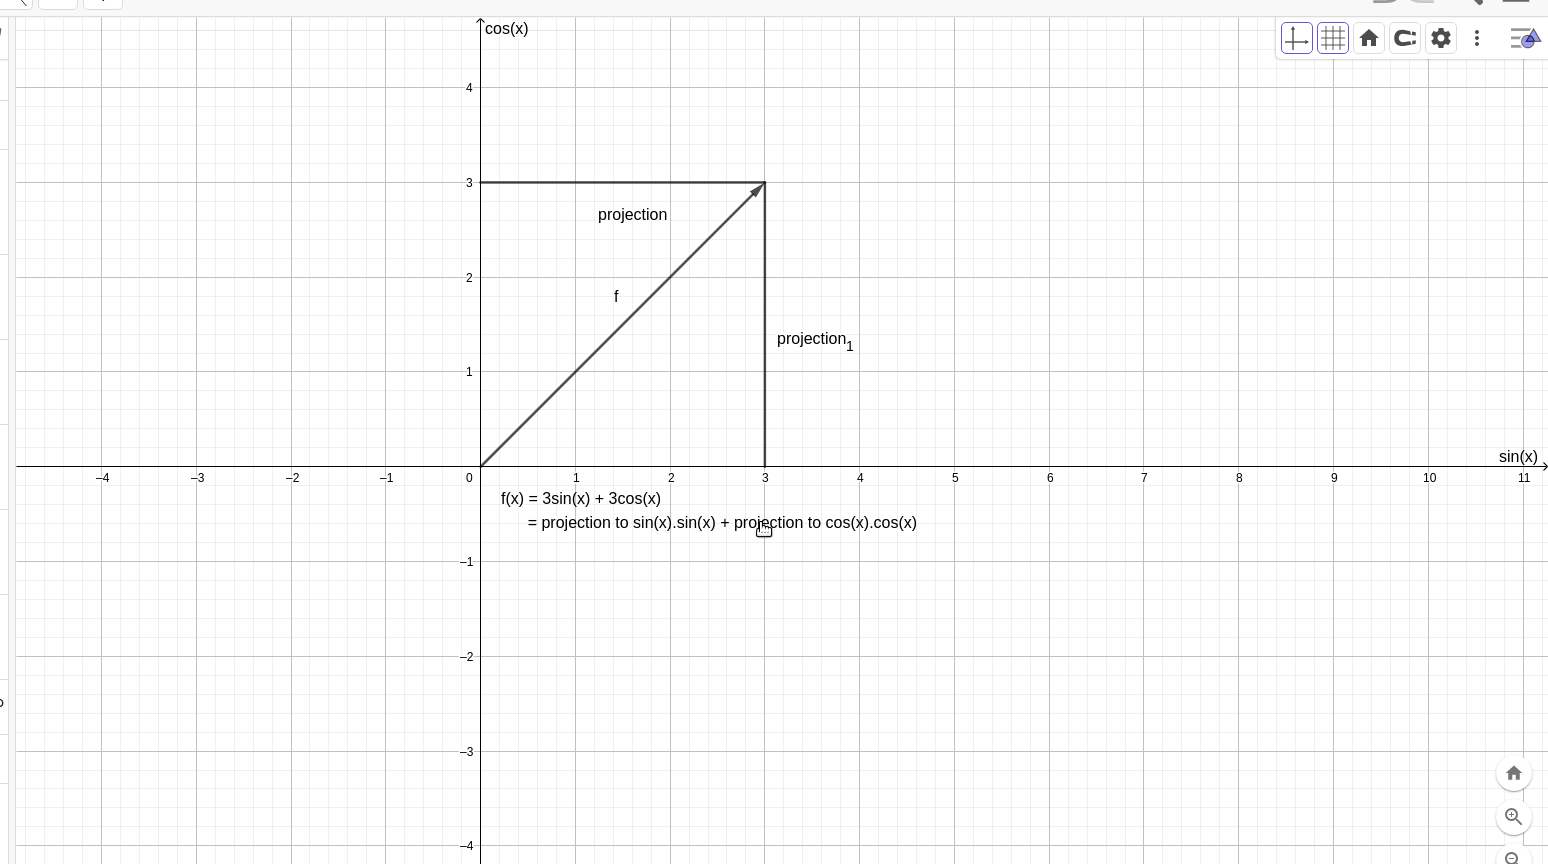
\includegraphics[width=.9\linewidth]{./ggv.png}
\end{center}
\subsection{Matlab}
\label{sec:org17bae97}
\begin{verbatim}
clear all, close all, clc

kmax = 7;

dx = 0.001;
L = pi;
x = (-1+dx:dx:1)*L;
f = 0*x;
n = length(f);
nquart = floor(n/4);
nhalf = floor(n/2);

f(nquart:nhalf) = 4*(1:nquart+1)/n;
f(nhalf+1:3*nquart) = 1-4*(0:nquart-1)/n;
subplot(3,1,1)
plot(x,f,'-','Color',[0 0 0],'LineWidth',1.5)
ylim([-.2 1.5])
xlim([-1.25*L 1.25*L])
set(gca,'LineWidth',1.2)
set(gca,'XTick',[-L 0 L],'XTickLabels',{});%{'-L','0','L','2L'})
set(gca,'YTick',[0 1],'YTickLabels',{});
box off

CC = colormap(jet(8));
% CCsparse = CC(5:5:end,:);
% CCsparse(end+1,:) = CCsparse(1,:);
CCsparse = CC(1:3:end,:);
%
subplot(3,1,2)
L = pi;
A0 = sum(f.*ones(size(x)))*dx;
plot(x,A0+0*f,'-','Color',CC(1,:)*.8,'LineWidth',1.2);
hold on
fFS = A0/2;
for k=1:kmax
    A(k) = sum(f.*cos(pi*k*x/L))*dx;
    B(k) = sum(f.*sin(pi*k*x/L))*dx;
    plot(x,A(k)*cos(k*pi*x/L),'-','Color',CC(k,:)*.8,'LineWidth',1.2);
%     plot(x,B(k)*sin(2*k*pi*x/L),'k-','LineWidth',1.2);
    fFS = fFS + A(k)*cos(k*pi*x/L) + 0*B(k)*sin(k*pi*x/L);
end
ylim([-.7 .7])
xlim([-1.25*L 1.25*L])
set(gca,'LineWidth',1.2)
set(gca,'XTick',[-L 0 L],'XTickLabels',{});%{'-L','0','L','2L'})
set(gca,'YTick',[-.5 0 .5],'YTickLabels',{});
box off
% 
subplot(3,1,1)
hold on
plot(x,fFS,'-','Color',CC(7,:)*.8,'LineWidth',1.2)
l1=legend('     ','    ')
set(l1,'box','off');
l1.FontSize = 16;


subplot(3,1,3)
A0 = sum(f.*ones(size(x)))*dx;
plot(x,A0+0*f,'-','Color',CC(1,:),'LineWidth',1.2);
hold on
fFS = A0/2;
for k=1:7
    Ak = sum(f.*cos(pi*k*x/L))*dx;
    Bk = sum(f.*sin(pi*k*x/L))*dx;
    plot(x,Ak*cos(k*pi*x/L),'-','Color',CC(k,:)*.8,'LineWidth',1.2);
%     plot(x,Bk*sin(2*k*pi*x/L),'k-','LineWidth',1.2);
    fFS = fFS + Ak*cos(k*pi*x/L) + 0*Bk*sin(k*pi*x/L);
end
ylim([-.06 .06])
xlim([-1.25*L 1.25*L])
set(gca,'LineWidth',1.2)
set(gca,'XTick',[-L 0 L],'XTickLabels',{});%{'-L','0','L','2L'})
set(gca,'YTick',[-.05 0 .05],'YTickLabels',{});
box off

set(gcf,'Position',[100 100 550 400])
set(gcf,'PaperPositionMode','auto')
print('-depsc2', '-loose', '../figures/FourierTransformSines');

%% Plot amplitudes
clear ERR
clear A
fFS = A0/2;
A(1) = A0/2;
ERR(1) = norm(f-fFS);
kmax = 100;
for k=1:kmax
    A(k+1) = sum(f.*cos(2*pi*k*x/L))*dx*2/L;
    B(k+1) = sum(f.*sin(2*pi*k*x/L))*dx*2/L;
%     plot(x,B(k)*sin(2*k*pi*x/L),'k-','LineWidth',1.2);
    fFS = fFS + A(k+1)*cos(2*k*pi*x/L) + 0*B(k+1)*sin(2*k*pi*x/L);
    ERR(k+1) = norm(f-fFS)/norm(f);
end
thresh = median(ERR)*sqrt(kmax)*4/sqrt(3);
r = max(find(ERR>thresh));
r = 7;
subplot(2,1,1)
semilogy(0:1:kmax,A,'k','LineWidth',1.5)
hold on
semilogy(r,A(r+1),'bo','LineWidth',1.5)
xlim([0 kmax])
ylim([10^(-7) 1])
subplot(2,1,2)
semilogy(0:1:kmax,ERR,'k','LineWidth',1.5)
hold on
semilogy(r,ERR(r+1),'bo','LineWidth',1.5)
xlim([0 kmax])
ylim([3*10^(-4) 20])
set(gcf,'Position',[100 100 500 300])
set(gcf,'PaperPositionMode','auto')
% print('-depsc2', '-loose', '../figures/FourierTransformSinesERROR');


\end{verbatim}
\section{Fourier Transform}
\label{sec:org1dbe9df}
\begin{itemize}
\item Fourier series is for periodic signals
\item If signal is not periodic then we can't use fourier series
\item Fourier transform is limiting case of fourier series when L \(\to\) \(\infty\)
\end{itemize}
\subsection{FT}
\label{sec:org296793f}
\begin{itemize}
\item \[ f(x) = \frac{1}{2\pi} \int_{-\infty}^{\infty} F(\omega)e^{j\omega x} dx \]
\item \[ F(\omega) = \int_{-\infty}^{infty} f(x)e^{-j\omega x} d\omega \]
\end{itemize}
\subsection{Work in progress}
\label{sec:org12d647e}
\section{Descrete Fourier Transform}
\label{sec:org7226e7b}
\begin{itemize}
\item In real life the data sould be in measuremnts in some time
\item We get time series insted of nice continues function
\item So the descrete fourier transform is descritized version of fourier transform
\end{itemize}
\subsection{DFT}
\label{sec:orgfbea701}
\begin{itemize}
\item In dft the integration become summation
\item DFT
\item F(k) = \(\sum_{n=0}^{N-1}\) f\(_{\text{n}}\) e\(^{\text{-2}\pi\ \text{n }\frac{k}{N}}\)
\item k \(\in\) 0 to N-1
\end{itemize}
\subsection{Inverse DFT}
\label{sec:org5dc4842}
\begin{itemize}
\item To come back to time series
\item f(n) = \(\sum_{k=0}^{N-1}\) F\(_{\text{k}}\) e\(^{\text{2}\pi\ \text{k }\frac{n}{N}}\)
\item n \(\in\) 0 to N-1
\end{itemize}
\subsection{DFT}
\label{sec:org084b162}
\begin{itemize}
\item let \(\omega_{\text{n}}\) = e\(^{\text{-j}\frac{2\pi}{N}}\)
\item Then we can reprasent DFT in matrix form
\end{itemize}
\subsection{Matrics form}
\label{sec:orgfcf4720}
\[ \begin{pmatrix} F_0\\F_1\\ \vdots \\F_{n-1} \end{pmatrix} = \begin{bmatrix}
1 & 1 & \ldots & 1 \\
1 & \omega & \ldots & \omega^{N-1} \\
\vdots & \vdots & \vdots & \vdots \\
1 & \omega^{n-1} & \ldots & \omega^{(N-1)^2} 
\end{bmatrix} \begin{pmatrix} f_0 \\ f_1 \\ \vdots \\ f_{N-1} \end{pmatrix} \]
\subsection{Beauty of matrices}
\label{sec:org66e5bbc}
\begin{itemize}
\item DFT matrix
\item \[ \begin{bmatrix} 1 & 1 & \ldots & 1 \\ 1 & \omega & \ldots & \omega^{N-1} \\ \vdots & \vdots & \vdots & \vdots \\ 1 & \omega^{n-1} & \ldots & \omega^{(N-1)^2} \end{bmatrix} \]
\end{itemize}
\subsection{Matlab code for DFT matrix}
\label{sec:org84ceb14}
\begin{verbatim}
clear all, close all, clc
n = 256;
w = exp(-i*2*pi/n);

% Slow
for i=1:n
    for j=1:n
	DFT(i,j) = w^((i-1)*(j-1));
    end
end

% Fast
[I,J] = meshgrid(1:n,1:n);
DFT = w.^((I-1).*(J-1));
imagesc(real(DFT))

\end{verbatim}
\subsection{Matlab Gibbs phenomena}
\label{sec:org14c79c0}
\begin{verbatim}
clear all, close all, clc

kmax = 7;

dx = 0.001;
L = pi;
x = (-1+dx:dx:1)*L;
f = 0*x;
n = length(f);
nquart = floor(n/4);
nhalf = floor(n/2);

f(nquart:nhalf) = 4*(1:nquart+1)/n;
f(nhalf+1:3*nquart) = 1-4*(0:nquart-1)/n;
subplot(3,1,1)
plot(x,f,'-','Color',[0 0 0],'LineWidth',1.5)
ylim([-.2 1.5])
xlim([-1.25*L 1.25*L])
set(gca,'LineWidth',1.2)
set(gca,'XTick',[-L 0 L],'XTickLabels',{});%{'-L','0','L','2L'})
set(gca,'YTick',[0 1],'YTickLabels',{});
box off

CC = colormap(jet(8));
% CCsparse = CC(5:5:end,:);
% CCsparse(end+1,:) = CCsparse(1,:);
CCsparse = CC(1:3:end,:);
%
subplot(3,1,2)
L = pi;
A0 = sum(f.*ones(size(x)))*dx;
plot(x,A0+0*f,'-','Color',CC(1,:)*.8,'LineWidth',1.2);
hold on
fFS = A0/2;
for k=1:kmax
    A(k) = sum(f.*cos(pi*k*x/L))*dx;
    B(k) = sum(f.*sin(pi*k*x/L))*dx;
    plot(x,A(k)*cos(k*pi*x/L),'-','Color',CC(k,:)*.8,'LineWidth',1.2);
%     plot(x,B(k)*sin(2*k*pi*x/L),'k-','LineWidth',1.2);
    fFS = fFS + A(k)*cos(k*pi*x/L) + 0*B(k)*sin(k*pi*x/L);
end
ylim([-.7 .7])
xlim([-1.25*L 1.25*L])
set(gca,'LineWidth',1.2)
set(gca,'XTick',[-L 0 L],'XTickLabels',{});%{'-L','0','L','2L'})
set(gca,'YTick',[-.5 0 .5],'YTickLabels',{});
box off
% 
subplot(3,1,1)
hold on
plot(x,fFS,'-','Color',CC(7,:)*.8,'LineWidth',1.2)
l1=legend('     ','    ')
set(l1,'box','off');
l1.FontSize = 16;


subplot(3,1,3)
A0 = sum(f.*ones(size(x)))*dx;
plot(x,A0+0*f,'-','Color',CC(1,:),'LineWidth',1.2);
hold on
fFS = A0/2;
for k=1:7
    Ak = sum(f.*cos(pi*k*x/L))*dx;
    Bk = sum(f.*sin(pi*k*x/L))*dx;
    plot(x,Ak*cos(k*pi*x/L),'-','Color',CC(k,:)*.8,'LineWidth',1.2);
%     plot(x,Bk*sin(2*k*pi*x/L),'k-','LineWidth',1.2);
    fFS = fFS + Ak*cos(k*pi*x/L) + 0*Bk*sin(k*pi*x/L);
end
ylim([-.06 .06])
xlim([-1.25*L 1.25*L])
set(gca,'LineWidth',1.2)
set(gca,'XTick',[-L 0 L],'XTickLabels',{});%{'-L','0','L','2L'})
set(gca,'YTick',[-.05 0 .05],'YTickLabels',{});
box off

set(gcf,'Position',[100 100 550 400])
set(gcf,'PaperPositionMode','auto')
print('-depsc2', '-loose', '../figures/FourierTransformSines');

%% Plot amplitudes
clear ERR
clear A
fFS = A0/2;
A(1) = A0/2;
ERR(1) = norm(f-fFS);
kmax = 100;
for k=1:kmax
    A(k+1) = sum(f.*cos(2*pi*k*x/L))*dx*2/L;
    B(k+1) = sum(f.*sin(2*pi*k*x/L))*dx*2/L;
%     plot(x,B(k)*sin(2*k*pi*x/L),'k-','LineWidth',1.2);
    fFS = fFS + A(k+1)*cos(2*k*pi*x/L) + 0*B(k+1)*sin(2*k*pi*x/L);
    ERR(k+1) = norm(f-fFS)/norm(f);
end
thresh = median(ERR)*sqrt(kmax)*4/sqrt(3);
r = max(find(ERR>thresh));
r = 7;
subplot(2,1,1)
semilogy(0:1:kmax,A,'k','LineWidth',1.5)
hold on
semilogy(r,A(r+1),'bo','LineWidth',1.5)
xlim([0 kmax])
ylim([10^(-7) 1])
subplot(2,1,2)
semilogy(0:1:kmax,ERR,'k','LineWidth',1.5)
hold on
semilogy(r,ERR(r+1),'bo','LineWidth',1.5)
xlim([0 kmax])
ylim([3*10^(-4) 20])
set(gcf,'Position',[100 100 500 300])
set(gcf,'PaperPositionMode','auto')
% print('-depsc2', '-loose', '../figures/FourierTransformSinesERROR');


\end{verbatim}
\subsection{Work in progres}
\label{sec:orgd47e096}
\section{FFT}
\label{sec:org6d8052f}
\begin{itemize}
\item FFT is anlgorithm to compute DFT fast and efficiently
\item It uses symetry in DFT
\item To compute DFT Without FFT it require O(n\(^{\text{2}}\)) but FFT require only O(nlog(n))
\end{itemize}
\subsection{}
\label{sec:orgbf37007}
\section{Gabor Transform}
\label{sec:orgf83598e}
\subsection{Limitations of Fourier transform}
\label{sec:org036d8d9}
\begin{itemize}
\item FT is good for repreasenting smooth signal when there is sudden jump or discontinuity then it is not capture very well Gibbs phenomena
\item FT is good for stationary signal
\item Stationary means frequency of signal not change with time
\item When we compute Fourier Transform we loss all of time information so we can't say when this frequency occured
\item non stationary signals example is audio signal which frequency changes with time
\end{itemize}

\subsection{Gabor transform}
\label{sec:org9c94832}
\begin{itemize}
\item it solve the problem of FT
\item Gabor Transfom allow us to compute spectrogram a time frequency plot
\item Also called windowed FT
\item We take a window function multiply with the signal and translate the signal to get gabor transform
\end{itemize}
\subsection{Gabor transform}
\label{sec:org5a270ad}
\begin{itemize}
\item pull out both time and frequency content
\item instead of computinf FT of entire signal we devide into several sections and compute FT of each section
\item Mathamaticaly we can write
\item \[ G(f(t)) = \int_{\infty}^{\infty} f(\tau)e^{-i \omega \tau} g(\tau - t) d \tau \]
\item g is the window function it can be gaussian or rectangular
\item We can't know what frequency exist at what time instead but we can know what frequency band exist at what time
\end{itemize}
\subsection{picture}
\label{sec:orgefbfc4f}
\begin{itemize}
\item gabor grid
\item \url{./gab.gif}
\end{itemize}
\subsection{Problems of gabor transform}
\label{sec:orgf4261a7}
\begin{itemize}
\item Uncertainity principle
\item It tells about when when you narrow the window you get better time resalution but you get poor frequency resalution
\item when you stretch the window you get better frquency inforation but poor time information
\item uncertainity principle tell us
\item \(\Delta\) t \(\Delta\) f \(\ge\) \(\frac{1}{4 \pi}\)
\end{itemize}
\subsection{matlab code for spectrogram}
\label{sec:orgc220ed6}
\begin{verbatim}
clear all, close all, clc

n = 128;
L = 30;
dx = L/(n);
x = -L/2:dx:L/2-dx;
f = cos(x).*exp(-x.^2/25);                    % Function
df = -(sin(x).*exp(-x.^2/25) + (2/25)*x.*f);  % Derivative

%% Approximate derivative using finite Difference...
for kappa=1:length(df)-1
    dfFD(kappa) = (f(kappa+1)-f(kappa))/dx;
end
dfFD(end+1) = dfFD(end);

%% Derivative using FFT (spectral derivative)
fhat = fft(f);
kappa = (2*pi/L)*[-n/2:n/2-1];
kappa = fftshift(kappa);  % Re-order fft frequencies
dfhat = i*kappa.*fhat;
dfFFT = real(ifft(dfhat));

%% Plotting commands
plot(x,df,'k','LineWidth',1.5), hold on
plot(x,dfFD,'b--','LineWidth',1.2)
plot(x,dfFFT,'r--','LineWidth',1.2)
legend('True Derivative','Finite Diff.','FFT Derivative')

\end{verbatim}
\subsection{beethoven code matlab}
\label{sec:org6280a8e}
\begin{verbatim}
clear all, close all, clc

% If you download mp3read, you can use this code
% also, need to download mp3read from 
% http://www.mathworks.com/matlabcentral/fileexchange/13852-mp3read-and-mp3write
% [Y,FS,NBITS,OPTS] = mp3read('../../DATA/beethoven.mp3'); % add in your own song
% T = 40;            % 40 seconds
% y=Y(1:T*FS);       % First 40 seconds
load ../../DATA/beethoven_40sec.mat 
%% Spectrogram
spectrogram(y,5000,400,24000,24000,'yaxis');

%% SPECTROGRAM 
% uncomment remaining code and download stft code by M.Sc. Eng. Hristo Zhivomirov
% wlen = 5000;
% h=400;        % Overlap is wlen - h
% % perform time-frequency analysis and resynthesis of the original signal
% [S, f, t_stft] = stft(y, wlen, h, FS/4, FS);  % y axis range goes up to 4000 HZ
% imagesc(log10(abs(S)));
% load CC.mat
% colormap(ones(size(CC))-(CC))
% 
% axis xy, hold on
% XTicks = [1 300 600 900 1200 1500 1800 2100];
% XTickLabels = {'0','5','10','15','20','25','30','35'};
% YTicks = [0 1000 2000 3000];
% YTickLabels = {'0','4000','8000','12000'};
% set(gca,'XTick',XTicks,'XTickLabels',XTickLabels);
% set(gca,'YTick',YTicks,'YTickLabels',YTickLabels);
% 
% % plot a frequency
% freq = @(n)(((2^(1/12))^(n-49))*440);
% freq(40) % frequency of 40th key = C

\end{verbatim}
\subsection{Idea}
\label{sec:org4942606}
\begin{center}
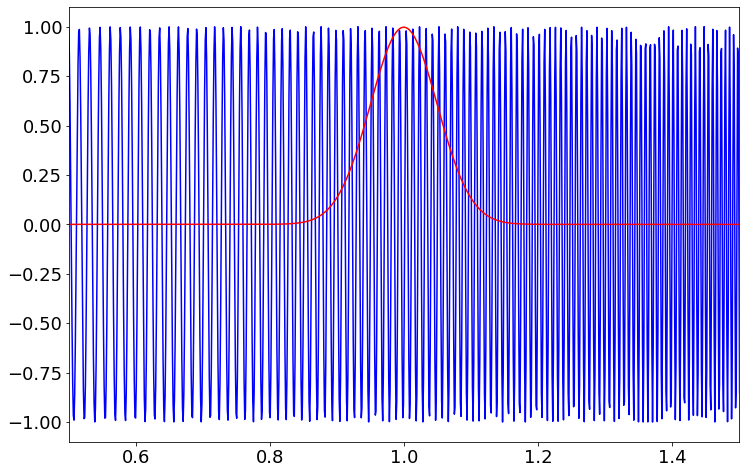
\includegraphics[width=.9\linewidth]{./gabor.png}
\end{center}
\section{Wavelet Transform}
\label{sec:orgd9abf7d}
\begin{itemize}
\item supercharged Fourier transform
\item Generalize Fourier transform
\item Reprasent signals interms of other orthogonal functions
\item 
\end{itemize}
\subsection{Wavelet}
\label{sec:org0d62c18}
\begin{itemize}
\item Wavelets are new basis functions also act as window function
\item Wavelets are some wave like oscilationg functions in limited durations
\item There are somany wavelets are avialable
\end{itemize}
\subsection{Haar Wavelet}
\label{sec:org00683c1}
\end{document}